\documentclass[11pt,a4paper]{article}
% \documentclass{book}

\setlength{\topmargin}{-0.5in}
\oddsidemargin = 15pt
%\marginparwidth = 15pt
\textwidth = 420pt
\setlength{\textheight}{10in}

\usepackage{url}
\usepackage{amsmath, amssymb}
\usepackage[ruled,linesnumbered]{algorithm2e}
\usepackage{bm}
\usepackage{multirow}
\usepackage{graphicx}
\usepackage{titling}
\usepackage[ampersand]{easylist}
\usepackage{enumitem}
\usepackage{subfigure}

\newcommand{\subtitle}[1]{%
  \posttitle{%
    \par\end{center}
    \begin{center}\large#1\end{center}
    \vskip0.5em}%
}
\newcommand{\includeMyGraphic}[1]{\includegraphics[clip=true, viewport=60 190 550 590, width=0.3\textwidth]{#1}}

\newlength{\wideitemsep}
\setlength{\wideitemsep}{0.5\itemsep}
\addtolength{\wideitemsep}{-5pt}
\let\olditem\item
\renewcommand{\item}{\setlength{\itemsep}{\wideitemsep}\olditem}

\newtheorem{prop}{Proposition}

\def \E    {\mathbb{E}}
\def \b    {\mathbf{b}}
\def \g    {\mathbf{g}}
\def \hy   {\widehat{y}}
\def \ty   {\widetilde{y}}
\def \f    {\mathbf{f}}
\def \x    {\mathbf{x}}
\def \Nn   {\mathcal{N}}
\def \Mu   {\pmb{\mu}}
\def \w    {\mathbf{w}}
\def \L    {\mathcal{L}}
\def \sign {\mathrm{sign}}
\def \I    {\mathbb{I}}

\newcommand{\dataset}{{\cal D}}
\newcommand{\fracpartial}[2]{\frac{\partial #1}{\partial  #2}}

\usepackage{listings}
\usepackage{xcolor}

\definecolor{mygreen}{rgb}{0,0.6,0}
\definecolor{mygray}{rgb}{0.5,0.5,0.5}
\definecolor{mygray2}{rgb}{0.9,0.9,0.9}
\definecolor{mymauve}{rgb}{0.58,0,0.82}

\lstset{ %
  backgroundcolor=\color{mygray2},   % choose the background color; you must add \usepackage{color} or \usepackage{xcolor}
  basicstyle=\footnotesize,        % the size of the fonts that are used for the code
  breakatwhitespace=true,         % sets if automatic breaks should only happen at whitespace
  %breaklines=true,                 % sets automatic line breaking
  captionpos=b,                    % sets the caption-position to bottom
  commentstyle=\color{mygreen},    % comment style
  keywordstyle=\color{blue},       % keyword style
  showspaces=false,                % show spaces everywhere adding particular underscores; it overrides 'showstringspaces'
  showstringspaces=false,          % underline spaces within strings only
  showtabs=false,                  % show tabs within strings adding particular underscores
  stringstyle=\color{mymauve},     % string literal style
  tabsize=4,                       % sets default tabsize to 2 spaces
  xleftmargin=-1.5cm,
  framexleftmargin=-1.5cm
}

\begin{document}

% Comment out these three lines to get the minimal LaTeX document
\title{\LARGE\textsf{SOL}: A Large Scale Sparse Online Learning Library}

\subtitle{Version 0.1.0}

\author{}

\maketitle

\begin{abstract}%   <- trailing '%' for backward compatibility of .sty file
    \textsf{SOL} is an open-source library for large-scale sparse online learning,
    which consists of a family of efficient and scalable sparse online learning
    algorithms for large-scale online  classification tasks. We have offered
    easy-to-use command-line tools and examples for users and developers. We also
    have made comprehensive documents available for both beginners and advanced
    users. SOL is not only a machine learning tool, but also a comprehensive
    experimental platform for conducting large scale sparse online learning research.
\end{abstract}

\newpage
\tableofcontents

\newpage

\section{Introduction}

Sparse online learning represents a family algorithms which try to explore
structure of features and learn a sparse model. It is valuable in handling
extremely large scale high dimensional datasets, which cannot be loaded into
memory.  The problem has been widely studied in batch learning, which is
effective but not scalable to large scale high dimensional data. Over the past
years, a variety of online learning algorithms have been proposed to explore
sparsity and maintain the benefits of online algorithms. However, there is very
few comprehensive libraries which include most of the state-of-the-art
algorithms for researchers to make easy side-by-side comparisons and for
developers to explore their various applications.

In this work, we develop \textsf{SOL}, an easy-to-use sparse online learning
tool that consists of a family of existing and recent state-of-the-art sparse
online learning algorithms for large-scale sparse online classification tasks.
SOL enjoys significant advantages for massive-scale classification in the era of big data nowadays, especially in efficiency,  scalability, and adaptability. 


\subsection{Problem Formulation}
The focus of sparse online learning is an algorithmic framework for regularized
convex programming to the following minimization problem:
\begin{equation}
    \min_{w}{f(w)} \qquad \qquad s.t. \qquad \qquad r(w) < R,
    \label{equ:obj0}
\end{equation}
where both $f(w)$ and $r(w)$ are convex bounded below functions. Often, $f(w)$
is an empirical loss and takes the form of $\sum_{i=1}^t{l_i}$ for a sequence
of loss functions $l_i$. $r(w)$ is a regularization term and often takes the
form of $\textit{L1}$ $(r(w) = |w|)$ or $\textit{L0}$ $(r(w) = |w|_0)$ norm.
$R$ is a pre-defined threshold to control sparsity of the model. With
lagrangian multiplier method, equation~\eqref{equ:obj0} can be reformulated as:
\begin{equation}
    \min_{w}{f(w) + \lambda r(w)}
    \label{equ:obj}
\end{equation}

\subsection{Summary of Main Algorithms}
Table~\ref{tab:summary-algorithms} gives a summary of the family of implemented algorithms in this software package. 

\begin{table}[!htpb]
    \caption{Summary of the Implemented Algorithms.}
    \label{tab:summary-algorithms}
%\begin{center}
    \begin{small}
        \renewcommand{\arraystretch}{1.3}
        \begin{tabular}{l||c|l|l}
            \hline
            Problem Type   &  Methodology & Algorithm & Description \\\hline \hline
            \multirow{12}{*}{Binary} &\multirow{4}{*}{\footnotesize First-Order}
            & SGD & {\footnotesize Stochastic Gradient Descent~\cite{rosenblatt1958perceptron}} \\\cline{3-4}
            & & STG & {\footnotesize Truncated sparse online learning~\cite{langford2009sparse}} \\\cline{3-4}
            & &FOBOS & {\footnotesize Forward backward splitting~\cite{duchi2009efficient}}\\\cline{3-4}
            & &RDA & {\scriptsize Regularized dual averaging~\cite{xiao2010dual}} \\\cline{2-4}
            &\multirow{8}{*}{\footnotesize Second-Order}
            &Ada-FOBOS & {\footnotesize Adaptive FOBOS~\cite{duchi2011adaptive}}\\\cline{3-4}
            &Classification  & Ada-RDA &Adaptive regularized dual averaging~\cite{duchi2011adaptive}\\\cline{3-4}
            & &AROW & Confidence weighted learning~\cite{crammer2009adaptive}\\\cline{3-4}
            & &AROW-TG & Confidence weighted truncated gradient\\\cline{3-4}
            & &AROW-DA & Confidence weighted dual averaging\\\cline{3-4}
            & &AROW-FS & Confidence weighted feature selection\\\cline{3-4}
            & &SCW & Soft confidence weighted learning~\cite{wang2012exact}\\\cline{3-4}
            & &SCW-RDA & Soft confidence weighted dual averaging\\\cline{3-4}
            \hline
        \end{tabular}
%\end{center}
    \end{small}
    \renewcommand{\arraystretch}{1}
\end{table}


\subsection{Main Features}
\begin{itemize}
    \item \textbf{Comprehensiveness:}
        A family of existing sparse online binary algorithms have been implemented in this software package;
    \item \textbf{Extendibility:}
        One can easily implement a new algorithm by only inheriting from a base
        class and implementing the key updating virtual functions.
    \item \textbf{Scalability:}
        The library can handle million and even billion scale dataset on a
        single PC.
    \item \textbf{Usability:}
        It is easy to use the main functions to evaluate one algorithm by comparing with all the algorithms;
\end{itemize}



\section{Installation}
SOL features a very simple installation procedure. No third-party dependencies
are required. The project is managed by \emph{CMake}. There
exists a \emph{CMakeLists.txt} in the root directory of SOL. Note that all the
following are tested on \emph{CMake 2.8}. Lower versions of cmake may work, but
are not ensured. 

\subsection{Installation on Linux}
The following steps have been tested for Ubuntu 12.04 but should work with
other distros as well.

\vspace{2mm}\hspace{-5mm}\textbf{Required Packages}

\begin{itemize}[leftmargin=1cm]
    \item GCC 4.6.2 or later. This can be installed with 
        \lstset{language=bash,
        }
        \begin{lstlisting}
        sudo apt-get install build-essential
        \end{lstlisting}
    \item CMake 2.8 or higher
    \item Python 2.7 
\end{itemize}


\hspace{-5mm}\textbf{Build from source}
\begin{enumerate}
    \item Create a temporary directory, which we denote as
        ($<$\emph{cmake\_binary\_dir}$>$), where you want to put the generated
        Makefiles, project files, as well the object files and output binaries.
    \item Enter the ($<$\emph{cmake\_binary\_dir}$>$) and type 
        \lstset{language=bash,
            framexleftmargin=-1.5cm,
        }
        \begin{lstlisting}
        cmake [<some optional parameters>] <path to SOL source directory>
        \end{lstlisting}

        For example
        \lstset{language=bash,
        }
        \begin{lstlisting}
        cd SOL
        mkdir build
        cd build
        cmake -DCMAKE_INSTALL_PATH=/usr/local/ ..
        \end{lstlisting}

    \item Enter the created temporary directory ($<$\emph{cmake\_binary\_dir}$>$) and proceed with: 
        \lstset{language=bash}
        \begin{lstlisting}
        make 
        make install
        \end{lstlisting}
\end{enumerate}

By default, SOL is installed in the directory \emph{$<$cmake\_source\_dir$>$/install}.


\subsection{Install on Windows}
The following steps have been tested on Visual Studio 2010 and Visual Studio
2012 on Windows 7 SP1. Nevertheless but should work with any other modern
versions of Visual Studio and Windows OS.

\vspace{2mm}\hspace{-5mm}\textbf{Required Packages}
\begin{itemize}
    \item Visual Studio 2010, 2012, or higher
    \item CMake 2.8 or higher
    \item Python 2.7 
\end{itemize}

\hspace{-5mm}\textbf{Build from source}
\begin{enumerate}
    \item Create a temporary directory, which we denote as
        ($<$\emph{cmake\_binary\_dir}$>$), where you want to put the generated
        project files as well the object files and output binaries.
    \item Install with CMake GUI.
        \begin{enumerate}
            \item Open \emph{cmake-gui.exe}, set where is the
                source code and where to build the binaries ($<$\emph{cmake\_binary\_dir}$>$).
                \begin{figure}[!h]
                    \centering
                    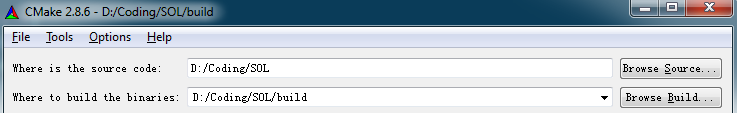
\includegraphics[width=0.8\textwidth]{figs/gui_path.png}
                    \label{fig:gui_path}
                \end{figure}
            \item Click \emph{Add Entry} and set install path. Otherwise, SOL will
                be install in ($<$\emph{cmake source directory}$>/install$).
                \begin{figure}[!h]
                    \centering
                    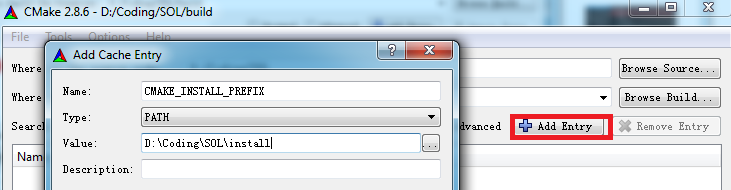
\includegraphics[width=0.8\textwidth]{figs/gui_install_path.png}
                    \label{fig:gui_install_path}
                \end{figure}

            \item Click \emph{Configure} and select compiler.
            \item After finish configuration, click \emph{Generate}.
                \begin{figure}[!h]
                    \centering
                    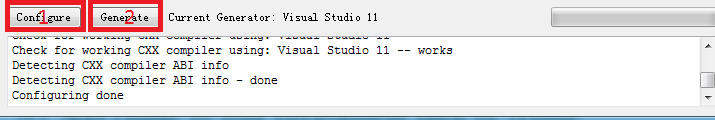
\includegraphics[width=0.8\textwidth]{figs/cmake_configure.png}
                    \label{fig:config}
                \end{figure}

            \item Open \emph{SOL.sln}, Rebuild all the \emph{ALL\_BUILD} project
                and then build \emph{INSTALL} project.
                \begin{figure}[!h]
                    \centering
                    \subfigure{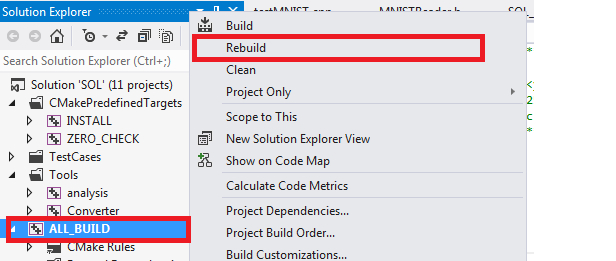
\includegraphics[width=0.4\textwidth]{figs/rebuild.png}}
                    \subfigure{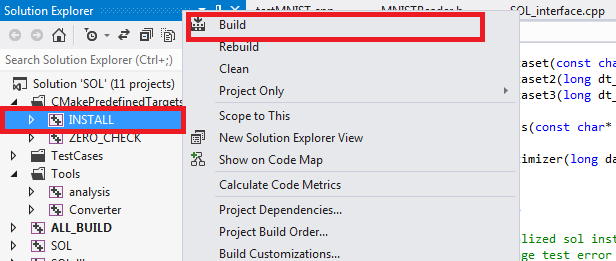
\includegraphics[width=0.4\textwidth]{figs/install.png}}
                    \label{fig:build}
                \end{figure}

        \end{enumerate}

    \item Install from command line. 
        
        Before this step, you should make sure that cmake is in the environment path or set environment path manually
        as step (c) shows.
        \begin{enumerate}
            \item Search \emph{cmd} in {Start Menu} and open it
            \item enter ($<$\emph{cmake\_binary\_dir}$>$)
            \item Add cmake to your environment path by typing:
                \lstset{language=bash,
                    framexleftmargin=-3cm,
                    xleftmargin=-3cm,
                }
                \begin{lstlisting}
                set path=%path%;<path_to_cmake>
                \end{lstlisting}
            \item generate Visual Studio Projects. Example code for Visual Studio
                2010 and 2012 are as the following shows:
                \lstset{language=bash,
                }
                \begin{lstlisting}
                #Generate Visual Studio 2010 Projects
                cmake  -G ``Visual Studio 10'' <path to SOL source directory>
                #Generate Visual Studio 2012 Projects
                cmake  -G ``Visual Studio 11'' <path to SOL source directory>
                \end{lstlisting}

                \begin{figure}[!h]
                    \centering
                    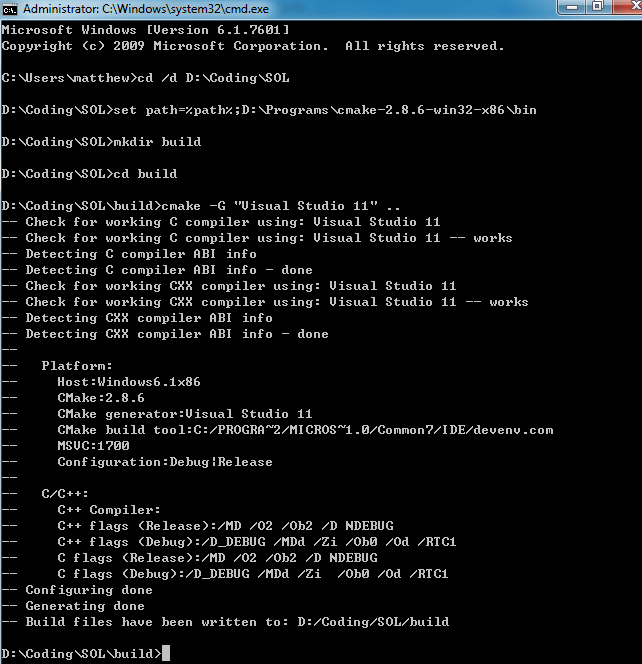
\includegraphics[width=0.8\textwidth]{figs/cmd.png}
                    \label{fig:cmd}
                \end{figure}
            \item Open \emph{SOL.sln}, Rebuild all the \emph{ALL\_BUILD} project
                and then build \emph{INSTALL} project.
        \end{enumerate}

\end{enumerate}


\section{How to Use the SOL Package}
The current version of SOL package are written in C++, with some python
scripts. The library is packed into an executable, a dynamic library, and a
static library. Some test cases are provided as examples.  

\subsection{Data Formats and Folders}

Types of data formats supported by this software package  are ``libsvm'' data
format (commonly used in LIBSVM and SVM-light), and a binary format defined by
ourselves. Features in the ``libsvm'' data files should all be numeric and labels are restricted to $+1, -1, 1$ for binary
classification.

\begin{itemize}
%\vspace{2mm}\hspace{-5mm}\textbf{Format of binary format}
    \item \textbf{Format of binary format}

        The binary format is for fast loading and processing. It is used to cache
        datasets. Each sample in binary format is comprised of the following
        items in sequence:
        \begin{itemize}
            \item \textbf{label}: sizeof(char)
            \item \textbf{feature number}: sizeof(char)
            \item \textbf{max index}: sizeof(int32\_t)
            \item \textbf{length of compressed index}: sizeoof(unsigned int) 
            \item \textbf{compressed index}: dynamic 
            \item \textbf{features}: feature number * sizeof(float)
            \item \textbf{sum of feature square}: sizeof(float)
        \end{itemize}

%\hspace{-5mm}\textbf{Contents of the library}:
    \item \textbf{Contents of the library}:

        \begin{itemize}
            \item   \textbf{data}: example datasets 
            \item   \textbf{doc}: documentation of the library
            \item   \textbf{exp}: python and matlab scripts for experiments, including cross validation and performance evaluation
            \item   \textbf{src}: source code of the library
            \item   \textbf{test}: test code and example use of the library
            \item   \textbf{tools}: python scripts to pre-process datasets
            \item   CMakeLists.txt
        \end{itemize}

\end{itemize}

\subsection{Command Line}
Running SOL without any arguments or with '-help/-h' will produce a message which briefly explains each argument. Below arguments are grouped according to their function.

\begin{enumerate}
    \item \textbf{Input Options}
        \begin{lstlisting}
            -i  arg :    training file name
            -c  arg :    cached training file name
            -t  arg :    test file name
            -tc arg :    cached test file name
            -dt arg :    dataset type format, by default is libsvm 
            -bs arg :    number of chunks for buffering, default is 2
        \end{lstlisting}

    \item \textbf{Loss Functions}
        \begin{lstlisting}
        -loss   arg :      loss function type
        \end{lstlisting}

        supported loss functions: 
        \begin{lstlisting}
        Hinge       :   hinge loss
        Logit       :   logistic loss
        Square      :   square loss
        SquareHinge :   squared hinge loss
        \end{lstlisting}

    \item \textbf{Learning Rate Setting:} Learning rate in our library is as the following equation shows:
        \begin{equation}
            \eta_t=\frac{\eta_0}{(t_0+t)^p}
            \label{equ:lrate}
        \end{equation}

        
        \begin{lstlisting}
        -eta     arg :  learning rate
        -power_t arg :  power t of decaying learning rate
        -t0      arg :  initial iteration number
        \end{lstlisting}

    \item \textbf{Algorithms and parameters}
        \begin{lstlisting}
        -opt    arg :   optimization method: 
                        SGD, STG, RDA, RDA_E, FOBOS Ada-RDA, Ada-FOBOS, 
                        AROW, AROW-TG, AROW-DA AROW-FS,SCW, SCW-RDA
        -l1     arg :   L1 regularization parameter
        -norm       :   whether normalize the data, default is false
        -passes arg :   number of passes 
        -delta  arg :   delta in Adaptive algorithms(Ada-)
        -grou   arg :   gamma times rou in enhanced RDA (RDA_E)
        -k      arg :   number of k in truncated gradient descent or 
                        feature selection
        -phi    arg :   phi in SCW
        -r      arg :   r in Confidence weighted algorithms
        \end{lstlisting}

        Table~\ref{tbl:param_illustrate} shows the algorithms and their
        correspondent parameters.  
        \begin{table}[!ht]
% increase table row spacing, adjust to taste
            \renewcommand{\arraystretch}{1.3}
 %\extrarowheight 
            \caption{Comparison of sparse online learning algorithms}
            \label{tbl:param_illustrate}
            \centering
            \begin{tabular}{|c|c|p{9cm}|}
                \hline
                Algorithm & Parameters & Meaning\\
                \hline
                SGD & -eta & learning rate \\
                \hline
                FOBOS & -eta & learning rate \\
                \hline
                \multirow{2}{*}{STG}& -eta & learning rate \\
                \cline{2-3}
                &-k & truncate the weight vector every k steps \\
                \hline
                \multirow{2}{*}{Ada-FOBOS}& -eta & learning rate \\
                \cline{2-3}
                & -delta & parameter to ensure positive-definite property of the adaptive weighting matrix \\
                \hline
                AROW-TG& -r &  parameter of passive-aggressive update trade-off\\
                \hline
                \multirow{2}{*}{RDA}&  -eat &  learning rate \\
                \cline{2-3}
                &-grou & decreased L1 regularization parameter \\
                \hline
                RDA\_E&  -eta & learning rate \\
                \hline
                \multirow{2}{*}{Ada-RDA}& -eta & learning rate \\
                \cline{2-3}
                & -delta & parameter to ensure positive-definite property of the adaptive weighting matrix \\
                \hline
                AROW-DA& -r  &parameter of passive-aggressive update trade-off\\
                \hline
                AROW-FS & -k & no default\\
                \hline
                \multirow{2}{*}{SCW}& -phi & probability parameter in SCW\\
                \cline{2-3}
                & -r & parameter of passive-aggressive update trade-off\\
                \hline
                \multirow{2}{*}{SCW-RDA}& -phi & probability parameter in SCW\\
                \cline{2-3}
                & -r & parameter of passive-aggressive update trade-off\\
                \hline
            \end{tabular}
        \end{table}
\end{enumerate}

\subsection{Use Command Line}
In this section, we show how to use the command line from terminals. We provide
an example to show how to use SOL and explain the details of how SOL works. The
dataset we use is rcv1.

Command for training is as the following.
\lstset{language=bash,
framexleftmargin=0.5cm,
xleftmargin=0.5cm,
}
\begin{lstlisting}
./SOL -i data/rcv1/rcv1.train -c  data/rcv1/rcv1.train_cache 
      -t data/rcv1/rcv1.test  -tc data/rcv1/rcv1.test_cache
\end{lstlisting}

For meaning of the input parameters, please refer to the explanation above.
Output of the above command will be:
\lstset{language=bash}
\begin{lstlisting}
--------------------------------------------------
Algorithm: SGD

Learning Rate: 10
Initial t  : 1
Power t : 0.5
lambda  : 0

Iterate No.             Error Rate
2                       0.500000
4                       0.500000
8                       0.500000
16                      0.437500
32                      0.531250
64                      0.515625
128                     0.515625
256                     0.417969
512                     0.341797
1024                    0.252930
2048                    0.182617
4096                    0.148193
8192                    0.122681
16384                   0.102661
32768                   0.090027
65536                   0.079849
131072                  0.072670
262144                  0.066559
524288                  0.061661
data number: 781265
Learn error rate: 5.97 +/- 0.00 %
Test error rate: 5.70 %
Sparsification Rate: 19.65 %
Learning time: 21.154 s
Test time: 0.530 s
\end{lstlisting}

\textbf{Illustrations}:
\begin{itemize}
    \item \emph{Algorithm}: this line is name of the algorithm applied to the dataset.
        By default, the algorithm is SGD. Select different algorithm by
        \emph{-opt $<$algorithm name$>$}. 
    \item \emph{Learning Rate}: $\eta_0$ in equation~\eqref{equ:lrate}. Change
        this value by \emph{-eta $<$val$>$}.
    \item \emph{Power t}: $p$ in equation~\eqref{equ:lrate}. Change this value
        by \emph{-power\_t $<$val$>$}.
    \item \emph{lambda}: $\lambda$ in equation~\eqref{equ:obj}. Change this
        value by \emph{-l1 $<$val$>$}. Note that this value will have no effect on
        SGD.
    \item \emph{data number}: number of samples in training data.
    \item \emph{Learn error rate}: learning error rate at the last iteration.
    \item \emph{Test error rate}: test error rate on the test data.
    \item \emph{Sparsification rate}: ratio of zero elements in the learned
        model.
    \item \emph{Learning time}: time to train the model
    \item \emph{Test time}: time to test the model.
\end{itemize}

To show how $\lambda$ will effect sparsity and accuracy, we set the algorithm
to STG, and change the value of $\lambda$ as table~\ref{tbl:lambda_effect} shows.
The command line is:
\lstset{language=bash,}
\begin{lstlisting}
./SOL -i data/rcv1/rcv1_train -c  data/rcv1/rcv1_train_cache 
      -t data/rcv1/rcv1_test  -tc data/rcv1/rcv1_test_cache 
      -opt STG -l1 lambda
\end{lstlisting}

\begin{table}[!h]
    \label{tbl:lambda_effect}
    \centering
    \begin{tabular}{|c|c|c|c|}
        \hline
        $\lambda$ & Learning error rate & test error rate & sparsity \\
        \hline
        0 & 5.97 & 5.7 & 19.65 \\
        1e-8 & 5.97 & 5.69 & 19.7 \\
        1e-7 & 5.98 & 5.7 & 20.09 \\
        1e-6 & 5.98 & 5.7 & 30.09 \\
        1e-5 & 6.1 & 5.84 & 67.56 \\
        1e-4 & 7.23 & 7.24 & 90.41 \\
        1e-3 & 15.54 & 18.34 & 97.71 \\
        1e-2 & 41.7 & 42.65 & 99.85\\
        1e-1 & 47.51 & 46.59 & 99.96 \\
        1 & 47.51 & 46.59 & 99.96 \\
        \hline
    \end{tabular}
    \caption{Effect of sparsity on learning error rate and test error rate}
    \label{tab:effect_lambda}
\end{table}

\subsection{Dynamic \& Static Library Interface}
Interfaces of dynamic/static library are comprised of three parts:
initialization, training/testing, and finalization.

\hspace{-5mm}\textbf{Initialization of IO}
\vspace{2mm}

Initialization of IO means to create a object of dataset. Users can use 
path to a libsvm data file to initialize a dataset (the ``\emph{sol\_init\_dataset}''). Or users can customize a reader
and use it as the parameter (``\emph{sol\_init\_dataset2}'' and
``\emph{sol\_init\_dataset3}''). The parameter ``\emph{cache\_filename}'' is for
cached data files. The program will cache the dataset to the specified file, or
the program will use the cached data if it already exist. In case when users do
not want to cached files, set it to an empty string ``''.

\lstset{language=C++}
\begin{lstlisting}
long sol_init_dataset (const char* filename, const char* cache_filename, 
                       const char* dt_type, int passNum, int buf_size);
long sol_init_dataset2(long dt_reader, int passNum, int buf_size);
long sol_init_dataset3(long dt_reader, const char* cache_filename, 
                       int passNum, int buf_size);
\end{lstlisting}

Note that the type ``\emph{long}'' here is actually  a pointer.

\vspace{4mm}\hspace{-5mm}\textbf{Initialization of Loss Functions}
\vspace{2mm}

Loss functions can either be initialized from the library, or be
user-customized. The api provided by the library is
\lstset{language=C++}
\begin{lstlisting}
long sol_init_loss(const char* loss_type);
\end{lstlisting}
``\emph{loss\_type}'' can be ``Hinge'', ``Logit'', or ``SquaredHinge''.

User-customized loss functions can also be used, as long as it is inherited
from the base Class ``\emph{LossFunction}''. Please refer
to section~\ref{sec:loss_func} and section~\ref{sec:extend_loss_func} for more
details about how to implement customized loss functions.

\vspace{4mm}\hspace{-5mm}\textbf{Initialization of Optimizers}
\vspace{2mm}
\lstset{language=C++}
\begin{lstlisting}
long sol_init_optimizer(long dataset, long loss_func, 
                        int argc, const char** args);
\end{lstlisting}
``\emph{dataset}'', ``\emph{loss\_func}'' are initialized as mentioned above.
As the third and fourth parameters, it is the same as mentioned in
\textbf{Command Line}.

\vspace{4mm}\hspace{-5mm}\textbf{Training/Testing}
\vspace{2mm}

Parameters to train or test the model is simply the initialized optimizer.
Meaning of the rest parameters are:
\lstset{language=C++}
\begin{lstlisting}
void sol_train( long optimizer, float* l_errRate, float* var_errRate, 
float* sparse_rate, float* time_cost);
void sol_test ( long optimizer, long test_dataset,  
float* t_errRate, float* time_cost);
\end{lstlisting}


\begin{itemize}
    \item \emph{l\_errRate}: learning error rate
    \item \emph{var\_errRate}: variance learning error rate, not valid at the
        moment
    \item \emph{sparse\_rate}: sparsification rate of the trained model
    \item \emph{t\_errRate}: test error rate
    \item \emph{time\_cost}: time cost of training/testing
    \item \emph{test\_dataset}: test dataset, initialized the same as mentioned
        above.
\end{itemize}

\vspace{4mm}\hspace{-5mm}\textbf{Finalization}
\vspace{2mm}

Finalization is to release the initialized resources. The functions are:
\lstset{language=C++}
\begin{lstlisting}
void sol_release_dataset(long dataset);
void sol_release_loss(long loss_func);
void sol_release_optimizer(long optimizer);
\end{lstlisting}

\subsection{Use Dynamic \& Static Library on Windows}
SOL can be linked as a dynamic library. It is named as ``SOLdll.dll'' on
Windows.  Interface of the library is in \emph{``src/SOL\_interface.h''}.
Before going on, please make sure the directory \emph{``$<$sol\_install\_path$>$/bin''} is in your system
environment path. Otherwise, you may encounter the ``dll not found'' error.
In the following, I will show an example to use \emph{SOL} as dynamic or static
libraries on Visual Studio 2012.

\begin{enumerate}
    \item Create an empty Win32 C/C++ project.
        \begin{figure}[!h]
            \centering
            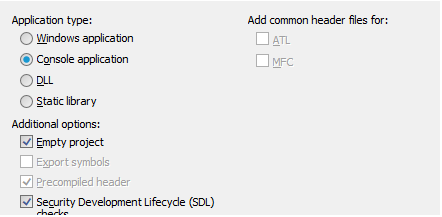
\includegraphics[width=0.8\textwidth]{figs/test_sol_new.png}
            \label{fig:test_sol_new}
        \end{figure}

    \item Add \emph{include} path and \emph{library} path to the created
        project. \emph{Properties} $\rightarrow$ \emph{Select All
        Configurations} $\rightarrow$ \emph{VC++ Directories}. 
        \begin{figure}[!h]
            \centering
            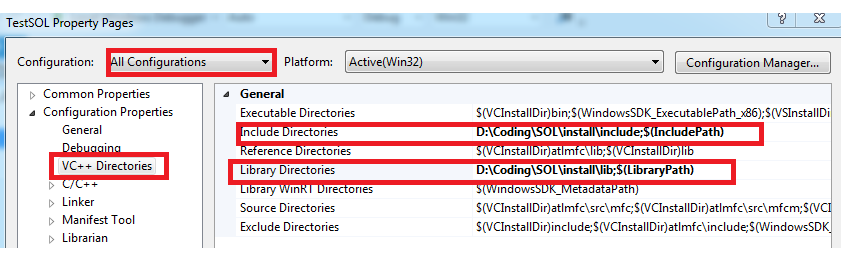
\includegraphics[width=0.8\textwidth]{figs/test_sol_config.png}
            \label{fig:test_sol_config}
        \end{figure}

    \item Add link libraries to the project. \emph{Linker} $\rightarrow$
        \emph{Input} $\rightarrow$ \emph{add the library}. In \emph{Release}
        mode, add \emph{SOLdll.lib} for dynamic library or \emph{SOLstatic.lib}
        for for static library. In \emph{Debug} mode, add \emph{SOLdlld.lib}
        for dynamic library or \emph{SOLstaticd.lib} for static library.
        \begin{figure}[!h]
            \centering
            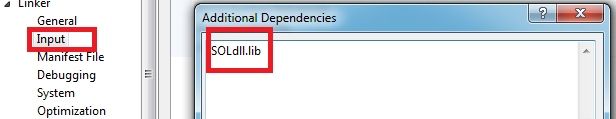
\includegraphics[width=0.8\textwidth]{figs/test_sol_linker.png}
            \label{fig:test_sol_linker}
        \end{figure}
    \item Test the program. Add a new source file and paste the following code to
        the file. You can copy the code from \emph{test/testDll/testDll.cpp}.
        Note that you may need to change the paths to training/test file.
        \lstset{language=C++, 
            framexleftmargin=-1cm,
            xleftmargin=-1cm,
        }
        \begin{lstlisting}
        #include "SOLdll.h"

        #include <iostream>
        #include <cstring>
        #include <vector>
        #include <cstdio>

        using namespace std;
        void release(long &dataset){
            sol_release_dataset(dataset);
            dataset = 0;
        }
        void release(long &dataset, long &loss_func){
            sol_release_dataset(dataset);
            sol_release_loss(loss_func);
            dataset = loss_func = 0;
        }
        void release(long &dataset, long &loss_func, long &opti){
            sol_release_dataset(dataset);
            sol_release_loss(loss_func);
            sol_release_optimizer(opti);
            dataset = loss_func = opti = 0;
        }

        int main(int argc, const char** args){
            printf("example: testDll [train_file test_file]\n");
            const char* train_file = "../../data/a7a/a7a";
            const char* test_file = "../../data/a7a/a7a.t";
            if(argc == 3){
                train_file = args[1];
                test_file = args[2];
            }

            vector<const char*> args_vec;
            args_vec.push_back("-opt");
            args_vec.push_back("AROW");

            long dataset = sol_init_dataset(train_file,"","libsvm",-1,-1);
            if (dataset == 0 ) {
                release(dataset);
                return -1;
            }
            long loss_func = sol_init_loss("hinge");
            if (loss_func == 0){
                release(dataset,loss_func);
                return -1;
            }
            long opti = sol_init_optimizer(dataset, loss_func,
                            args_vec.size(), &(args_vec[0]));
            if  (opti == 0){
                release(dataset, loss_func, opti);
                return -1;
            }

            float l_err(0), var_err(0), sparse_rate(0), time_cost(0);
            sol_train(opti,&l_err, &var_err, &sparse_rate, &time_cost);


            long t_dataset = sol_init_dataset(test_file,"","libsvm",-1,-1);
            if (t_dataset != 0){
                float t_errRate(0), t_cost(0);
                sol_test(opti,t_dataset,&t_errRate, &t_cost);
                sol_release_dataset(t_dataset);
                printf("Learn error rate: %.2f +/- %.2f %%\n",
                        l_err * 100, var_err * 100);
                printf("Test error rate: %.2f %%\n",t_errRate* 100); 
                printf("Sparsification Rate: %.2f %%\n", sparse_rate * 100);
                printf("Learning time: %.3f s\n", time_cost);
                printf("Test time: %.3f s\n", t_cost);
            }
            else{
                printf("Learn error rate: %.2f +/- %.2f %%\n",
                        l_err * 100, var_err * 100);
                printf("Sparsification Rate: %.2f %%\n", sparse_rate * 100);
                printf("Learning time: %.3f s\n", time_cost);
            }
            release(dataset, loss_func, opti);
            return 0;
        }

        \end{lstlisting}
\end{enumerate}

\subsection{Use Dynamic \& Static Library on Linux}
On linux, users need to set the include path, library link path, and linked
libraries in the \emph{makefile}. 
\begin{enumerate}
    \item Include path: 
        \lstset{language=C++, 
            framexleftmargin=-1.5cm,
            xleftmargin=-1.5cm,
        }   
        \begin{lstlisting}
        -I <sol install path>/include
        \end{lstlisting}
    \item Link path and library

        \textbf{Static Library}
        \lstset{language=bash}
        \begin{lstlisting}
        -L <sol install path>/lib -lSOLstatic
        \end{lstlisting}
        \textbf{Dynamic Library}
        \lstset{language=bash}
        \begin{lstlisting}
        -L <sol install path>/bin -lSOLdll
        \end{lstlisting}
\end{enumerate}

\lstset{language=C++, 
    framexleftmargin=-1cm,
    xleftmargin=-1cm,
}
\subsection{Use Scripts in experiments}
In the ``\emph{exp}'' folder, there are some scripts to help compare different
algorithms.
\begin{itemize}
    \item \emph{exe\_path.py}

        This file defines the path to executables. Users may need to change the
        path according to their installation.
    \item \emph{dataset.py}

        This file defines paths to dataset. Users can add and delete datasets
        as needed in function ``\emph{get\_file\_name}'' and
        ``\emph{get\_model\_param}''.  Note the ``\emph{rootDir}'' at the
        beginning of the file. Users need to change it to the root directory of
        datasets.

    \item \emph{CV.py}

        This  script is used to do cross validation. Usage of the script is:
        \lstset{language=python,
            framexleftmargin=-1cm,
            xleftmargin=-1cm,
        }
        \begin{lstlisting}
        python CV.py dataset_name algorithm fold_num param start:step:end
        \end{lstlisting}

        \textbf{Parameters:}
        \lstset{language=bash,
            framexleftmargin=-1cm,
            xleftmargin=-1cm,
        }

        \begin{lstlisting}
        dataset_name    : name of the dataset defined in dataset.py
        algorithm       : name of the algorithm
        fold_num        : number of folds to do cross validation
        param           : parameter to be cross validated. Note that this
        takes the form ``-eta'' as command line.
        start:step:end  : search space for the parameter.
        \end{lstlisting}

        \textbf{Notes:}
        \begin{itemize}
            \item \emph{param} and \emph{start:step:end} can appear more than
                one time. For example:
                \lstset{language=python,
                    framexleftmargin=-3cm,
                    xleftmargin=-3cm,
                }
                \begin{lstlisting}
                python CV.py rcv1 Ada-FOBOS 10 -eta 0.5:2:256 -delta 0.03125:2:32
                \end{lstlisting}
            \item Users may need to set the extra command in \emph{CV.py}.
                Currently, it is:
                \lstset{language=python}
                \begin{lstlisting}
                -loss Hinge -norm
                \end{lstlisting}

        \end{itemize}

    \item \emph{batch\_cv.py}

        Scripts to do cross validation in batch. What users need to do is to set the
        algorithm list ``\emph{opt\_list}'', dataset list
        ``\emph{ds\_list}'', and folder number ``\emph{fold\_num}''.

    \item \emph{l1\_def.py} 

        This file defines different sparse regularization parameters to different
        dataset and to different algorithms. Users may need to modify these
        files to get a full view of how sparsity will effect accuracy.

    \item \emph{demo.py}

        This script evaluates how sparsity will affect accuracy. Users need to
        set the algorithm list ``\emph{opt\_list}'', dataset list
        ``\emph{ds\_list}'', number of times to randomize the dataset. Advanced
        users can check other settings.

    \item \emph{draw.m}

        Matlab scripts to draw how test error rate is affected by sparsity.
    \item \emph{draw\_convergence.m}

        Matlab scripts to draw how convergence with iterations.
    \item \emph{draw\_time.m}

        Matlab scripts to draw how training time is affected by sparsity.
\end{itemize}

In the following, we show how sparsity will affect test error rate, convergence
, and training time for different algorithms. First, we obtain the parameters by
cross validation. Parameter setting in \emph{batch\_cv.py} is as the following
shows:
\lstset{language=python,
    framexleftmargin=-.5cm,
    xleftmargin=-0.5cm,
}
\begin{lstlisting}
    opt_list = ['RDA','Ada-RDA', 'CW-RDA']
    ds_list = ['rcv1']
    fold_num = 5
    
    eta_search = '0.5:2.0:512'
    delta_search = '0.03125:2:32'
    r_search = delta_search
\end{lstlisting}
Then we evaluate effect of sparsity.
\lstset{language=python}
\begin{lstlisting}
    opt_list = ['RDA','Ada-RDA', 'CW-RDA']
    ds_list = ['rcv1']
    #number of times to randomize a dataset for averaged results
    rand_num = 10
    #extra command sent to SOL
    extra_cmd = ' -loss Hinge -norm'
\end{lstlisting}

Results are as the following shows:
\begin{figure}[!h]
    \caption{Example of effect of sparsity}
    \centering
    \subfigure[test error rate]{ \includeMyGraphic{./figs/rcv1-DA-test-sparse.pdf}}
    \subfigure[convergence on 90\% sparsity]{ \includeMyGraphic{./figs/rcv1-DA-conv.pdf}}
    \subfigure[time cost]{ \includeMyGraphic{./figs/rcv1-DA-time-sparse.pdf}}
    \label{fig:rcv1_result}
\end{figure}


\subsection{Parameter Settings}

Setting proper parameters plays a nontrivial role in affecting the empirical
performance of different sparse online learning algorithms.
Table~\ref{tbl:algo_param} gives a summary of parameters and their
default settings by different sparse online learning algorithms. Note that we
do not include sparsity parameter $\lambda$ in this table.


To enable fair side-by-side comparisons between different algorithms, there are two
choices:
\begin{itemize}
    \item Enable the learn best parameter setting ``\emph{-lbp}'' in
        the command line. This scheme selects best parameters one after another
        if there are more than one parameters.
    \item Use the provided scripts to do cross validation.
\end{itemize}

\begin{table}[!h] \vspace{-5mm}
% increase table row spacing, adjust to taste
    \renewcommand{\arraystretch}{1.3}
 %\extrarowheight 
    \caption{Comparison of sparse online learning algorithms}
    \label{tbl:algo_param}
    \centering
    \begin{tabular}{|c|c|c|c|c|c|}
        \hline
        Algorithm & Norm & Type & Parameters \\
        \hline
        SGD & NA & First Order & $\eta = 10$ \\
        \hline
        FOBOS & L1 & First Order & $\eta = 10$ \\
        \hline
        STG& L1 & First Order & $\eta = 10, k = 10$\\
        \hline
        ADA-FOBOS & L1 & Second Order  & $\eta = 10, \delta = 10$ \\
        \hline
        AROW-TG& L1 & Second Order  & $r = 1$ \\
        \hline
        RDA& L1 & First Order & $\eta = 10$ \\
        \hline
        ADA-RDA& L1 & Second Order  & $\eta = 10, \delta = 10$ \\
        \hline
        AROW-DA& L1 & Second Order  & $r = 1$ \\
        \hline
        AROW-FS & L0 & Second Order  & $k$, no default\\
        \hline
    \end{tabular}
\end{table}

\section{System Framework}

The design principle is to keep the package simple, easy to read and extend.
All codes follow the C++99 standard and need no external libraries. The reason
to choose C++ is for feasibility and efficiency in handling large scale high
dimensional data. The system is designed so that machine learning researchers
can quickly implement a new algorithm with a new idea, and compare it with a
large family of existing algorithms without spending much time and efforts in
handling large scale data. We choose python to compare different algorithms as
it is more easy to read and it does not affect the performance of algorithms
themselves.

In general, SOL is written in a modular way, in which one can easily develop a
new algorithm and make side-by-side comparisons with the existing ones in the
package. Thus, we hope that SOL is not only a machine learning tool, but also a
comprehensive experimental platform for conducting sparse online learning research.

Figure~\ref{fig:framework} shows the framework of the system.
\begin{figure}[!ht]
    \centering
    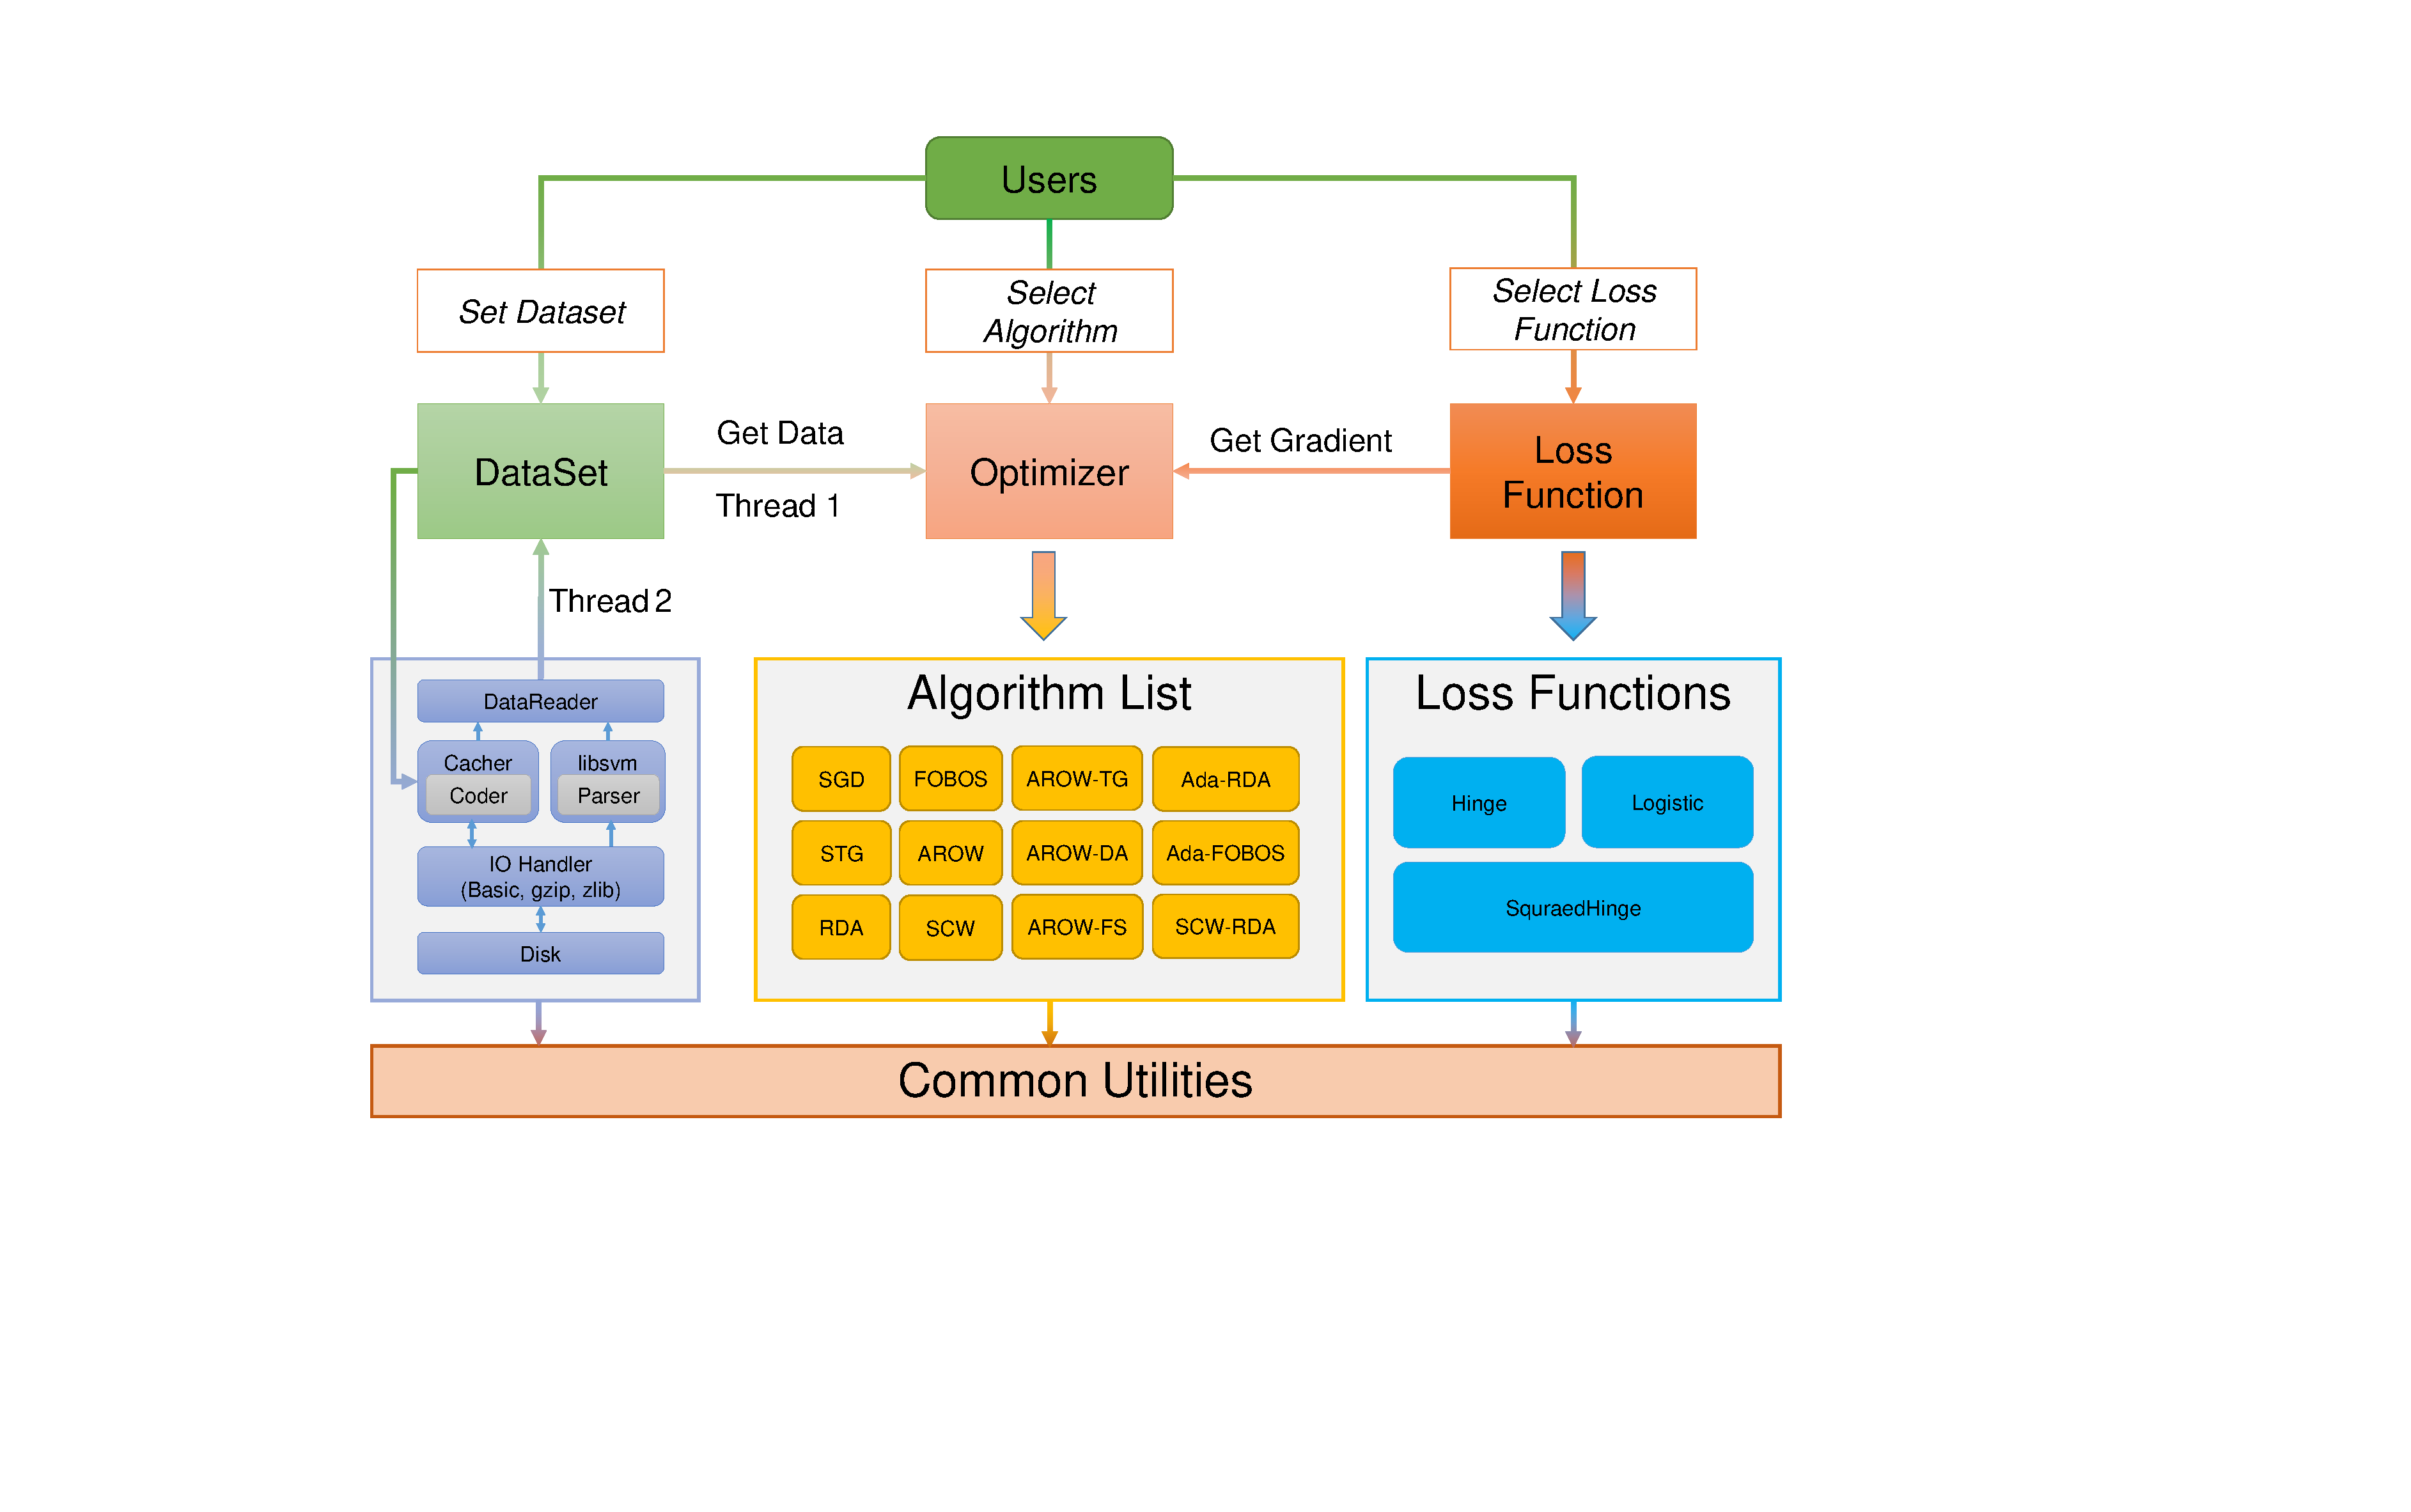
\includegraphics[width=0.9\textwidth]{figs/framework.pdf}
    \caption{Framework of SOL}
    \label{fig:framework}
\end{figure}

\subsection{DataSet}

DataSet is in charge of transfering data from disk to optimizers efficiently. The three major functions are: parsing the original dataset, caching data, and a common interface with optimizers.

\vspace{4mm}\hspace{-5mm}\textbf{Loading Data}
\vspace{2mm}

It requires dataset readers to parse different formats of data. By default, we
support \emph{libsvm} and the cached \emph{binary} format. Base class to parse
a dataset is \emph{DataReader} (in \emph{DataReader.h}), in which we define the
interfaces to load a dataset file correctly. The interfaces are:

\begin{itemize}
    \item \emph{OpenReading}:
        \lstset{language=C++,
            framexleftmargin=-1cm,
            xleftmargin=-1cm,
        }
        \begin{lstlisting}
        virtual bool OpenReading() = 0;
        \end{lstlisting}
        Open a dataset file to load data. Note that we do not specify the
        source of dataset (like a file path name). It is specified in the
        constructor to support diverse data sources. Source of data can be files, TCP, etc. The
        open operation can go beyond opening a local file. It can also open a
        socket listener.

        The function returns true if everything is ok.

    \item \emph{GetNextData}:
        \lstset{language=C++}
        \begin{lstlisting}
        virtual bool GetNextData(DataPoint<FeatType, LabelType> &data) = 0;
        \end{lstlisting}

        Get a new data point from the source. The parameter is the variable to place the obtained data.

        The function returns true if everything is ok.

    \item \emph{Rewind}:
        \lstset{language=C++}
        \begin{lstlisting}
        virtual void Rewind() = 0;
        \end{lstlisting}

        Rewind the data source to the beginning

    \item \emph{Close}:
        \lstset{language=C++}
        \begin{lstlisting}
        virtual void Close() = 0;
        \end{lstlisting}

        Close the data source when loading is finished.

    \item \emph{Good}:
        \lstset{language=C++}
        \begin{lstlisting}
        virtual bool Good() = 0;
        \end{lstlisting}

        Test if the data reader is ok. Note that end of file(eof) is
        \textbf{NOT} regared as \textbf{Bad} status.
\end{itemize}


\subsection{Loss Function}\label{sec:loss_func}

At the moment, we provide a base class (purely virtual class) for loss
functions and three inherited classes(\emph{HingleLoss}, \emph{Logit}, and
\emph{SquaredHinge}). The interfaces are:

\begin{itemize}
    \item \textbf{IsCorrect}:
        \lstset{language=C++,
            framexleftmargin=-1cm,
            xleftmargin=-1cm,
        }        \begin{lstlisting}
        virtual inline bool IsCorrect(LabelType label, float predict);
        \end{lstlisting}

        This function is implemented in the base class to justify whether a
        prediction is correct for binary classification problems. We assign the
        virtual property to it for the extensibility to multi-class or
        regression problems.

    \item \textbf{GetLoss}:
        \lstset{language=C++}
        \begin{lstlisting}
        virtual float GetLoss(LabelType label, float predict) = 0;
        \end{lstlisting}

        Get the loss of the current prediction

    \item \textbf{GetGradient}:
        \lstset{language=C++}
        \begin{lstlisting}
        virtual float GetGradient(LabelType label, float predict) = 0;
        \end{lstlisting}

        Get the gradient of the loss function at the current data point. Note that we do not calculate the exact gradient here. To linear classification problems, the gradients on different features share a same part. Take Hinge Loss for example:
        $$l(\vec{w}) = 1 - y\vec{w}\cdot\vec{x}$$
        The gradient is:
        $$l'(\vec{w}) = -y\vec{x}$$

        As a result, we only calculate the shared term $-y$ for the gradients
        of different features for efficiency concern. Users need to multiply
        the correspondent feature $x[i]$ in the optimization algorithms.
\end{itemize}

\subsection{Optimizers}
Optimizers are the sparse online learning algorithms. The base class Optimizer
implements the details of how a classification model works, including
interacting with a dataset, training the model, updating the model, test the
model, and some other auxiliary functions. It also define the interfaces for
different learning algorithms(the virtual functions).

\vspace{4mm}\hspace{-5mm}\textbf{Details of Optimizer class}
\vspace{2mm}

\begin{enumerate}
    \item \textbf{Variables}:

        \lstset{language=bash,
            framexleftmargin=-1.5cm,
            xleftmargin=-2cm,
        }
        \begin{lstlisting}
        eta0   : initial learning rate
        eta    : learning rates. This variable is set to eta0 at beginning.
        Different algorithms can set the value on the fly.
        id_str :  a string to describe the algorithm, need to be assigned a value 
        when an algorithm is constructed
        lambda :  The L1 regularization parameter.
        dataSet     : object of training data.
        lossFunc    : user specified loss function
        weightVec   : The weight vector of the linear model.
        weightDim   : current dimension of the weight vector. Note that 
        this variable is changing with training data coming in.
        initial_t   : initial iteration number, this is the variable to avoid 
        large learning rates at the beginning
        curIterNum  : current iteration number
        sparse_soft_thresh : threshold below which a weight is regarded as zero.
        \end{lstlisting}

    \item \textbf{Constructor}:

        \lstset{language=C++}
        \begin{lstlisting}
        Optimizer(DataSet<FeatType, LabelType> &dataSet, 
        LossFunc<FeatType, LabelType> &lossFunc); 
        \end{lstlisting}
        When initializing an optimizer, users need to assign the data set and
        the loss function. 

    \item \textbf{Training}:

        Following are the functions to learn a model.

        \begin{itemize}
            \item \textbf{Learn}: public function called by users to learn a
                model.
                \lstset{language=C++,
                    framexleftmargin=-2.8cm,
                    xleftmargin=-2.8cm,
                }
                \begin{lstlisting}
                float Learn(int numOfTimes = 1);
                \end{lstlisting}

                Learn a model and return the average error rate. Note that the input
                parameter is only used for those dataset that can be randomized, which is
                not available at the moment.

                \lstset{language=C++}
                \begin{lstlisting}
                float Learn(float &aveErrRate, float &varErrRate, 
                float& sparseRate, int numOfTimes = 1);
                \end{lstlisting}

                Learn a model and return the average error rate.

                \textbf{Parameters}:


                \lstset{language=C++}
                \begin{lstlisting}
                aveErrRate: average error rate
                varErrRate: variance of the average error rate, 
                only valid when dataset can be randomized
                sparesRate: sparsification rate of the linear model
                numOfTimes: number of times to learn the model with 
                randomized dataset, not available at the moment
                \end{lstlisting}

            \item \textbf{BeginTrain}:
                \lstset{language=C++}
                \begin{lstlisting}
                virtual void BeginTrain();
                \end{lstlisting}

                Reset the optimizer to the initialization status of training

                \textbf{Note}: If user-customized algorithm contains some new parameters
                that need to be reset, users should call this base function explicitly in their
                inherited function to ensure the model is reset correctly.

            \item \textbf{Train}:
                \lstset{language=C++}
                \begin{lstlisting}
                float Train();
                \end{lstlisting}

                Train the model and return the learning error rate.

            \item \textbf{EndTrain}:
                \lstset{language=C++}
                \begin{lstlisting}
                virtual void EndTrain();
                \end{lstlisting}

                Called when training is finished.

            \item \textbf{Predict}:

                \lstset{language=C++}
                \begin{lstlisting}
                float Predict(DataPoint<FeatType, LabelType> &data);
                \end{lstlisting}

                Predict the label of the input data point.

            \item \textbf{Update model}:

                \lstset{language=C++}
                \begin{lstlisting}
                virtual float UpdateWeightVec(
                const DataPoint<FeatType, LabelType> &x) = 0;
                \end{lstlisting}

                The core function of learning. This function is called each time a new data point comes to update the model.

                $\textbf{x}$: the new data that comes in

                The function returns prediction of the input data \textbf{x}.

        \end{itemize}
    \item \textbf{Test}

        \lstset{language=C++,
            framexleftmargin=-1.5cm,
            xleftmargin=-1.5cm,
        }
        \begin{lstlisting}
        float Test(DataSet<FeatType ,LabelType> &testSet);
        \end{lstlisting}

        Test the performance of the given dataset. Return the test error rate.

    \item \textbf{Auxiliary Function}
        \lstset{language=C++,
            framexleftmargin=-2.8cm,
            xleftmargin=-2.8cm,
        }
        \begin{itemize}
            \item \textbf{Set Parameters}:

                \lstset{language=C++}
                \begin{lstlisting}
                void SetParameter(float lambda = -1, float eta0 = -1);
                \end{lstlisting}

                Set the learning rate and L1 regularization parameter. -1 means no change.

            \item \textbf{Learn best parameter}:

                \lstset{language=C++}
                \begin{lstlisting}
                virtual void BestParameter();
                \end{lstlisting}

                Learn the best learning rate by default. It can be inherited and learn other parameters to satisfy the requirements of different algorithms.

            \item \textbf{get sparse rate}:

                \lstset{language=C++}
                \begin{lstlisting}
                float GetSparseRate(int total_len = 0);
                \end{lstlisting}

                Get the sparse rate of the model. The total\_len is the dimension of the input data. If not assigned by users, the largest index of features will be used.

            \item \textbf{update dimension of data}:

                \lstset{language=C++}
                \begin{lstlisting}
                virtual void UpdateWeigthSize(int newDim);
                \end{lstlisting}

                Update the dimension of the weight vector. As we are learning
                on sparse data online, we do not know the dimension of the
                input data. So the weight vector needs to be resized on the
                fly. Note that inherited algorithms need to overridden this
                function to resize their own dimension-related members and call
                the base one explicitly to resize the weight vector.

            \item \textbf{print algorithm info}

                \lstset{language=C++}
                \begin{lstlisting}
                void PrintOptInfo() const;
                \end{lstlisting}

                Print the optimization information.

            \item \textbf{Id\_Str}

                \lstset{language=C++}
                \begin{lstlisting}
                const string& Id_Str() const;
                \end{lstlisting}

                Get the identity string of the optimizer.
        \end{itemize}

\end{enumerate}

\subsection{How to Add New Algorithms}
A salient property of this library is that it provides a fairly easy-to-use
testbed to facilitate sparse online learning researchers to develop their new
algorithms and conduct side-by-side comparisons with the state-of-the-art
algorithms on various datasets with various loss functions with the minimal
efforts.  More specifically, adding a new algorithm has to address two major
issues:
\begin{itemize}
    \item What is the condition for making an update? This is usually equivalent to defining a proper loss function (e.g., a hinge loss $\mathrm{l\_t=max(0,1-y\_t*f\_t)}$) such that an update occurs wherever the loss is nonzero, i.e., $(l_t>0)$.

    \item How to perform the update on the classifier (i.e.,the weight vector $\mathbf{w}$) whenever the condition is satisfied? For example, Perceptron updates $w = w + y\_t*x_t$;

    \item Are there some parameters in your new algorithm? If so, you need to
        do some initializations, including (i) modify the
        "$\mathrm{init\_params.h}$" file by adding the initialization; (ii)
        override the ``$\mathrm{BestParameter.h}$" to learn best parameter as needed.
\end{itemize}


\subsection{Extend DataReader}

For a specific format of data, we only need to inherit from the
\emph{DataReader} class and implement the above interfaces. It will work when
you assign the customized data reader to the dataset.

The file \emph{libsvmread.h} and \emph{MNISTReader.h} (in ``\emph{testMNIST}''
folder) can be regarded as an example to extend \emph{DataReader}.

\subsection{Extend Loss Functions}\label{sec:extend_loss_func}
To implement a new loss function, users only need to inherit from the class
``\emph{LossFunction}'', and implement the pure virtual functions.  The files
\emph{HingeLoss.h}, \emph{LogisticLoss.h}, and \emph{SquareHingeLoss.h} are
three examples to extend the base class. 

\subsection{Implement your own algorithms}
To implement a specific learning algorithm, users only need to inherit from the
base class \emph{Optimizer}, and implement the pure virtual function
\emph{UpdateWeightVec}. Whether other virtual functions need to be override
depends on the specific algorithm. Take \emph{STG} for example, it has to
maintain a time stamp vector. So it override the \emph{BeginTrain} and
\emph{UpdateWeightSize} functions to initialize and resize the time stamp
vector. It needs to shrink weight vectors at the end of the training. So
\emph{EndTrain} is overridden.

Check the implemented algorithms to explore more details of how to extend the optimizers.

\section{Documentation}

The SOL package comes with comprehensive documentation. The README file describes the setup and usage. Users can read the ``Quick
Start" section to begin shortly. All the functions and related data structures are explained in detail. If the README file does not give the information
users want, they can also check this document and the software manual.

\newpage

\section{Conclusions, Revision, and Citation}
SOL is an easy-to-use open source package for efficient and scalable sparse
online linear classification. It is currently one of comprehensive online
learning software packages that include the largest number of diverse sparse
online learning algorithms for sparse online classification. SOL is still being improved by improvements from practical users and new research results~. The ultimate goal is to make easy learning with massive-scale data streams to tackle the emerging grand challenge of big data mining.

% Acknowledgements should go at the end, before appendices and references

\subsection*{Revision History}
\begin{itemize}
    \item{Version 0.1.0} was released on January 10th, 2014. This version
        mainly includes C++ implementation for binary classification. 
\end{itemize}

Welcome to send us your suggestions/corrections for SOL by the following email:
\begin{center}\url{chhoi@ntu.edu.sg}\end{center}

\subsection*{Citation}
In citing SOL in your papers, please use the following reference:\\

%S.C.H. Hoi, J. Wang, P. Zhao. LIBOL: A Library for Online Learning Algorithms. Nanyang Technological University, 2012.
%\url{http://LIBOL.stevenhoi.org}.

% Manual newpage inserted to improve layout of sample file - not
% needed in general before appendices/bibliography.

% Note: in this sample, the section number is hard-coded in. Following
% proper LaTeX conventions, it should properly be coded as a reference:

%In this appendix we prove the following theorem from
%Section~\ref{sec:textree-generalization}:

%{\noindent \em Remainder omitted in this sample. See http://www.jmlr.org/papers/ for full paper.}
%\vskip 0.2in
\bibliographystyle{abbrv}
\bibliography{reference}

\end{document}
